 % % Template for PLoS
% % Version 3.3 June 2016
% %
% % % % % % % % % % % % % % % % % % % % % % %
% %
% % -- IMPORTANT NOTE
% %
% % This template contains comments intended 
% % to minimize problems and delays during our production 
% % process. Please follow the template instructions
% % whenever possible.
% %
% % % % % % % % % % % % % % % % % % % % % % % % 
% %
% % Once your paper is accepted for publication, 
% % PLEASE REMOVE ALL TRACKED CHANGES in this file 
% % and leave only the final text of your manuscript. 
% % PLOS recommends the use of latexdiff to track changes during review, as this will help to maintain a clean tex file.
% % Visit https://www.ctan.org/pkg/latexdiff?lang=en for info or contact us at latex@plos.org.
% %
% %
% % There are no restrictions on package use within the LaTeX files except that 
% % no packages listed in the template may be deleted.
% %
% % Please do not include colors or graphics in the text.
% %
% % The manuscript LaTeX source should be contained within a single file (do not use \input, \externaldocument, or similar commands).
% %
% % % % % % % % % % % % % % % % % % % % % % % %
% %
% % -- FIGURES AND TABLES
% %
% % Please include tables/figure captions directly after the paragraph where they are first cited in the text.
% %
% % DO NOT INCLUDE GRAPHICS IN YOUR MANUSCRIPT
% % - Figures should be uploaded separately from your manuscript file. 
% % - Figures generated using LaTeX should be extracted and removed from the PDF before submission. 
% % - Figures containing multiple panels/subfigures must be combined into one image file before submission.
% % For figure citations, please use "Fig" instead of "Figure".
% % See http://journals.plos.org/plosone/s/figures for PLOS figure guidelines.
% %
% % Tables should be cell-based and may not contain:
% % - spacing/line breaks within cells to alter layout or alignment
% % - do not nest tabular environments (no tabular environments within tabular environments)
% % - no graphics or colored text (cell background color/shading OK)
% % See http://journals.plos.org/plosone/s/tables for table guidelines.
% %
% % For tables that exceed the width of the text column, use the adjustwidth environment as illustrated in the example
% % table in text below.
% %
% % % % % % % % % % % % % % % % % % % % % % % % %
% %
% % -- EQUATIONS, MATH SYMBOLS, SUBSCRIPTS, AND SUPERSCRIPTS
% %
% % IMPORTANT
% %
% % Below are a few tips to help format your equations and other special characters according to our specifications. For
% % more tips to help reduce the possibility of formatting errors during conversion, please see our LaTeX guidelines at
% % http://journals.plos.org/plosone/s/latex
% %
% % For inline equations, please be sure to include all portions of an equation in the math environment.  For example,
% % x$^2$ is incorrect; this should be formatted as $x^2$ (or $\mathrm{x}^2$ if the romanized font is desired).
% %
% % Do not include text that is not math in the math environment. For example, CO2 should be written as
% % CO\textsubscript{2} instead of CO$_2$.
% %
% % Please add line breaks to long display equations when possible in order to fit size of the column.
% %
% % For inline equations, please do not include punctuation (commas, etc) within the math environment unless this is part
% % of the equation.
% %
% % When adding superscript or subscripts outside of brackets/braces, please group using {}.  For example, change
% % "[U(D,E,\gamma)]^2" to "{[U(D,E,\gamma)]}^2".
% %
% % Do not use \cal for caligraphic font.  Instead, use \mathcal{}
% %
% % % % % % % % % % % % % % % % % % % % % % % % % 
% %
% % Please contact latex@plos.org with any questions.
% %
% % % % % % % % % % % % % % % % % % % % % % % % %

% \documentclass[10pt,letterpaper]{article}
% \usepackage[top=0.85in,left=2.75in,footskip=0.75in]{geometry}

% % amsmath and amssymb packages, useful for mathematical formulas and symbols
% \usepackage{amsmath,amssymb}

% % Use adjustwidth environment to exceed column width (see example table in text)
% \usepackage{changepage}

% % Use Unicode characters when possible
% \usepackage[utf8x]{inputenc}

% % textcomp package and marvosym package for additional characters
% \usepackage{textcomp,marvosym}

% % cite package, to clean up citations in the main text. Do not remove.
% \usepackage{cite}

% % Use nameref to cite supporting information files (see Supporting Information section for more info)
% \usepackage{nameref,hyperref}

% % line numbers
% \usepackage[right]{lineno}

% % ligatures disabled
% \usepackage{microtype}
% \DisableLigatures[f]{encoding = *, family = * }

% % color can be used to apply background shading to table cells only
% \usepackage[table]{xcolor}

% % array package and thick rules for tables
% \usepackage{array}

% % create "+" rule type for thick vertical lines
% \newcolumntype{+}{!{\vrule width 2pt}}

% % create \thickcline for thick horizontal lines of variable length
% \newlength\savedwidth
% \newcommand\thickcline[1]{%
%   \noalign{\global\savedwidth\arrayrulewidth\global\arrayrulewidth 2pt}%
%   \cline{#1}%
%   \noalign{\vskip\arrayrulewidth}%
%   \noalign{\global\arrayrulewidth\savedwidth}%
% }

% % \thickhline command for thick horizontal lines that span the table
% \newcommand\thickhline{\noalign{\global\savedwidth\arrayrulewidth\global\arrayrulewidth 2pt}%
% \hline
% \noalign{\global\arrayrulewidth\savedwidth}}


% % Remove comment for double spacing
% %\usepackage{setspace} 
% %\doublespacing

% % Text layout
% \raggedright
% \setlength{\parindent}{0.5cm}
% \textwidth 5.25in 
% \textheight 8.75in

% % Bold the 'Figure #' in the caption and separate it from the title/caption with a period
% % Captions will be left justified
% \usepackage[aboveskip=1pt,labelfont=bf,labelsep=period,justification=raggedright,singlelinecheck=off]{caption}
% \renewcommand{\figurename}{Fig}

% % Use the PLoS provided BiBTeX style
% \bibliographystyle{plos2015}

% % Remove brackets from numbering in List of References
% \makeatletter
% \renewcommand{\@biblabel}[1]{\quad#1.}
% \makeatother

% % Leave date blank
% \date{}

% % Header and Footer with logo
% \usepackage{lastpage,fancyhdr,graphicx}
% \usepackage{epstopdf}
% \pagestyle{myheadings}
% \pagestyle{fancy}
% \fancyhf{}
% \setlength{\headheight}{27.023pt}
% \lhead{\includegraphics[width=2.0in]{PLOS-submission.eps}}
% \rfoot{\thepage/\pageref{LastPage}}
% \renewcommand{\footrule}{\hrule height 2pt \vspace{2mm}}
% \fancyheadoffset[L]{2.25in}
% \fancyfootoffset[L]{2.25in}
% \lfoot{\sf PLOS}

% %% Include all macros below

% \newcommand{\cursedforest}{\textsc{CursedForest}\xspace}
% \newcommand{\ranger}{\textsc{Ranger}\xspace}
% \newcommand{\randomforest}{\textsc{randomForest}\xspace}
% \newcommand{\mtry}{\texttt{mtry}\xspace}
% \newcommand{\ntree}{\texttt{ntree}\xspace}

% %% END MACROS SECTION

% %% Additional packages
% \usepackage{footmisc}
% \usepackage{multirow}


% %%local edits (rob)
% \let\oldmarginpar\marginpar
% \renewcommand\marginpar[1]{\-\oldmarginpar[\raggedleft\footnotesize #1]%hv
% {\raggedright\footnotesize #1}}
% \reversemarginpar
% \setlength{\marginparwidth}{5cm}
% \usepackage{caption}
% \usepackage{subcaption}
% \usepackage{placeins}
% \usepackage{xspace} % see http://tex.stackexchange.com/questions/31091/space-after-latex-commands

% \begin{document}
% \vspace*{0.2in}

% % Title must be 250 characters or less.
% \begin{flushleft}
% {\Large
% \textbf\newline{The Donoho--Tanner Phase Change} % Please use "title case" (capitalize all terms in the title except conjunctions, prepositions, and articles).
% }
% \newline
% % Insert author names, affiliations and corresponding author email (do not include titles, positions, or degrees).
% Robert Dunne


% Insert additional author notes using the symbols described below. Insert symbol callouts after author names as necessary.
% 
% Remove or comment out the author notes below if they aren't used.
%
% Primary Equal Contribution Note
%\Yinyang These authors contributed equally to this work.

% Additional Equal Contribution Note
% Also use this double-dagger symbol for special authorship notes, such as senior authorship.
%\ddag These authors also contributed equally to this work.

% Current address notes
%\textcurrency a Insert current address of first author with an address update
% \textcurrency b Insert current address of second author with an address update
% \textcurrency c Insert current address of third author with an address update

% Deceased author note
%\dag Deceased

% Group/Consortium Author Note
%\textpilcrow Membership list can be found in the Acknowledgments section.

% Use the asterisk to denote corresponding authorship and provide email address in note below.

% \end{flushleft}




\documentclass[11pt]{article}

\usepackage{geometry}
 \geometry{
 a4paper,
% total={210mm,297mm}
% }
 left=17mm,
 right=23mm,
 top=20mm, 
 bottom=20mm,
}

\bibliographystyle{apalike}
\usepackage{url}
\usepackage{rotating}
\usepackage{natbib}
\usepackage{placeins}
\usepackage{longtable}
\usepackage[latin1]{inputenc}
\usepackage{multirow}
\usepackage{hyperref}
%\usepackage{showframe}
\usepackage{pdflscape}
%\usepackage{pbox}
\usepackage{xcolor}
\usepackage{amsmath}
\usepackage{rotating}
\usepackage{multicol}
\usepackage{caption}
\usepackage{subcaption}
\usepackage{xspace} % see http://tex.stackexchange.com/questions/31091/space-after-latex-commands


\usepackage{pdflscape}

\usepackage{listings}

\lstset{
  basicstyle=\ttfamily, 
  basewidth=0.5em,                 %the default setting of listings with "fixed columns" has a space 0.6em wide, 
                                   %while the characters in Computer Modern Typewriter are 0.5em wide.
                                   %http://tex.stackexchange.com/questions/179071/spacing-looks-wrong-in-listings-when-using-fixed-columns
  backgroundcolor=\color{gray!10},
  keywordstyle=\color{green!40!black},
  columns=fixed,
  language=R,                     % the language of the code
  basicstyle=\footnotesize,       % the size of the fonts that are used for the code
  numbers=left,                   % where to put the line-numbers
  numberstyle=\tiny\color{gray},  % the style that is used for the line-numbers
  stepnumber=1,                   % the step between two line-numbers. If it's 1, each line
                                  % will be numbered
  numbersep=5pt,                  % how far the line-numbers are from the code
  showspaces=false,               % show spaces adding particular underscores
  showstringspaces=false,         % underline spaces within strings
  showtabs=false,                 % show tabs within strings adding particular underscores
  frame=single,                   % adds a frame around the code
  rulecolor=\color{black},        % if not set, the frame-color may be changed on line-breaks within not-black text (e.g. commens (green here))
  tabsize=2,                      % sets default tabsize to 2 spaces
  captionpos=b,                   % sets the caption-position to bottom
  breaklines=true,                % sets automatic line breaking
  breakatwhitespace=false,        % sets if automatic breaks should only happen at whitespace
  title=\lstname,                 % show the filename of files included with \lstinputlisting;
                                  % also try caption instead of title
  keywordstyle=\color{blue},      % keyword style
  commentstyle=\color{green},   % comment style
  stringstyle=\color{red},      % string literal style
  escapeinside={\%*}{*)},         % if you want to add a comment within your code
  morekeywords={*,...}            % if you want to add more keywords to the set
} 

\usepackage{graphicx}
\usepackage{gensymb}
\usepackage{nag}   %It warns the user about the usage of old packages or commands (for example, using \it, \tt, etc.)
\usepackage{fixltx2e}
%fixltx2e package. It fixes some 'mistakes' in Latex. From the description:
%        ensure one-column floats don't get ahead of two-column floats;
%        correct page headers in twocolumn documents;
%        stop spaces disappearing in moving arguments;
%        allowing \fnysmbol to use text symbols;
%        allow the first word after a float to hyphenate;
%        \emph can produce caps/small caps text;
\usepackage{booktabs}
% \centering instead of \begin{center} \end{center} to center things inside tables/figures etc. \centering doesn't add any additional vertical space.
\usepackage{microtype}  %for small-scale typographic enhancements (character protrusion, font expansion, letter-spacing).
\usepackage{fancyvrb}   %get precise control in verbatim listings.
%\usepackage{siunitx} To typeset units
\usepackage{numprint} %format numbers nicely 
%~, the non-breakable space.

\parindent=0pt
\parskip=8pt
\setlength\itemsep{0em}

%\sloppy
%\SweaveOpts{echo=FALSE,prefix.string=script18/plot}
\renewcommand{\textfraction}{0.0}

\let\oldmarginpar\marginpar
\renewcommand\marginpar[1]{\-\oldmarginpar[\raggedleft\footnotesize #1]%
{\raggedright\footnotesize #1}}

\newcommand{\supp}{\mathop{\mathrm{supp}}}

\newcommand{\cursedforest}{{\sc CursedForest}}
\newcommand{\mtry}{{\texttt mtry}}
\newcommand{\ntree}{{\texttt ntree}}


\newsavebox\ltmcbox

\title{\cursedforest\ - A Random Forest Implementation for ``Big'' and ``Wide'' Data \\
Supplementary Information}
\author{}
\date{}



\begin{document}
%\setkeys{Gin}{width=8cm}
\setkeys{Gin}{height=8cm,width=0.9\columnwidth}
\maketitle
%%\tableofcontents
%% ## \begin{landscape}
%% ##   \small
%% ## \end{landscape}


%% \begin{lstlisting}
%% \end{lstlisting}





\section{supplementary Information for Section 4.1}




\section{intro}

We have demonstrated that using a different parallelization model can extend random forests to the case of an
extremely large number of variables. We have treated the case of variable selection in a $p >> n$ model where most of
the variables are uninformative and have demonstrated the utility of the model for large GWAS datasets. By comparing
this implementation to other implementations (including those optimized for large datasets) we have demonstrated the
utility of this approach.

Donoho and Tanner \cite{Donoho.and.Tanner.2009} give a ``universal phase change'' result that has applications in a
large number of areas including variable selection in high dimensions. They show that there is a sharp disjunction
between the cases where significant variables may be recovered with a high accuracy by procedures like stepwise variable
selection, and the cases where they can not be recovered. The boundary is shown in
Fig~\ref{figure:phase-diagram-equivalence.png} in a space parameterized by the level of underdeterminedness,
$\delta = n/p$, and by the sparsity, $\rho =k/n$ (where $k$ is the number of significant variables). The theoretical
boundary is based on arguments from combinatorial geometry. Above the phase-transition line variable recovery is still
possible by a combinatorial approach such as all-subsets variable selection. 




\begin{figure}[tbhp] 
    \centering
    \includegraphics[totalheight=6cm]{./figs/phase-diagram-equivalence.png} 
    \caption{{\bf The phase change diagram.}}
    \label{figure:phase-diagram-equivalence.png} 
    \vspace{4ex}
\end{figure}


\subsection{the simulation}
\cite{Donoho.and.Stodden.2006} investigate the behavior of a number of
regression approaches for variable selection in a small simulation.  They consider a regression probem with 
$\underset{n\times p}{X}\sim N(0,1)$ with $p$ fixed at 200 and $n$ variable.
They  set $\beta(1:k) \sim U(1,100)$ and $\beta((k+1):p) =0$. Then  $y= X\beta + \epsilon$, $\epsilon \sim
N(0,\sqrt{16})$. They evaluate variable selection by the error measure 
$$\frac{\Vert\hat{\beta}-\beta\Vert_2}{\Vert\beta\Vert_2}$$

They consider a number of variable selection methods, including a false discovery rate criteria. This involves adding
the variable with the maximum $t$-value to the linear model if the $p$-value is less than 
$25(\text{number of  terms  currently  in  the  model})/(\text{total  number  of  variables})$.  
See Fig~\ref{figure:error_Stodden_FDR.png} for the error measure and
figure \ref{figure:rbo_Stodden_FDR.png} for the RBO, comparing the ranking (i.e. values) of $\hat{\beta}$ and $\beta$.
It apparent that there is a marked drop in the accuracy of the variable recovery in line with the pediction of the
Donoho-Tanner phase transition.

\begin{figure}[tbhp] 
    \begin{subfigure} [b]{0.5\linewidth}
      \centering
      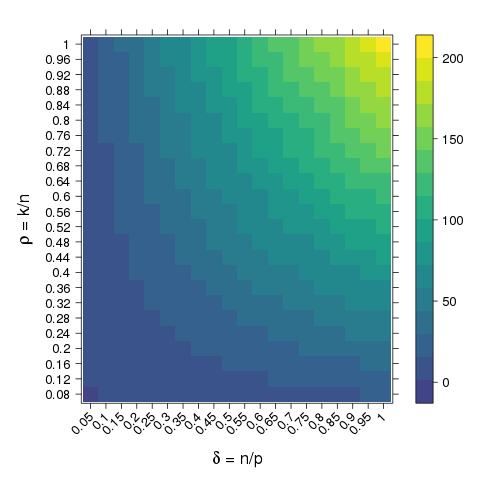
\includegraphics[totalheight=6cm]{./figs/k.png}
      \caption{$k$}
      \label{figure:k.png}
    \end{subfigure} 
    \begin{subfigure}[b]{0.5\linewidth}
      \centering
      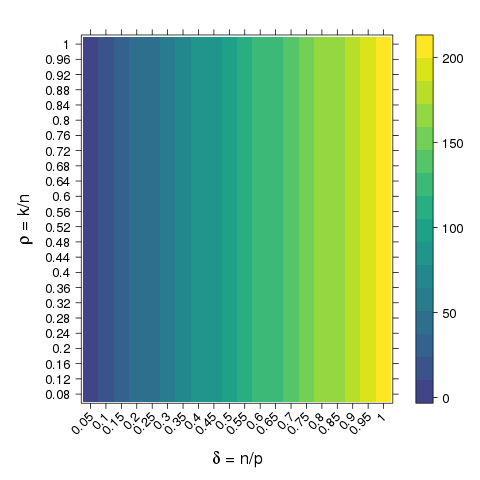
\includegraphics[totalheight=6cm]{./figs/n.png}
      \caption{$n$}
      \label{figure:n.png}
    \end{subfigure} 
    \caption{The simulation in \protect{\cite{Donoho.and.Stodden.2006}} considers $\delta = n/p$ and $\rho =k/n$. Here we plot the
      space of $\{ \delta, \rho$\}, colored  by the paramters $n$ and $k$}
\end{figure}


 \begin{figure}[tbhp] 
%   \begin{adjustwidth}{-1.00in}{0in}
     \begin{subfigure}[t]{0.5\linewidth}
       \centering
       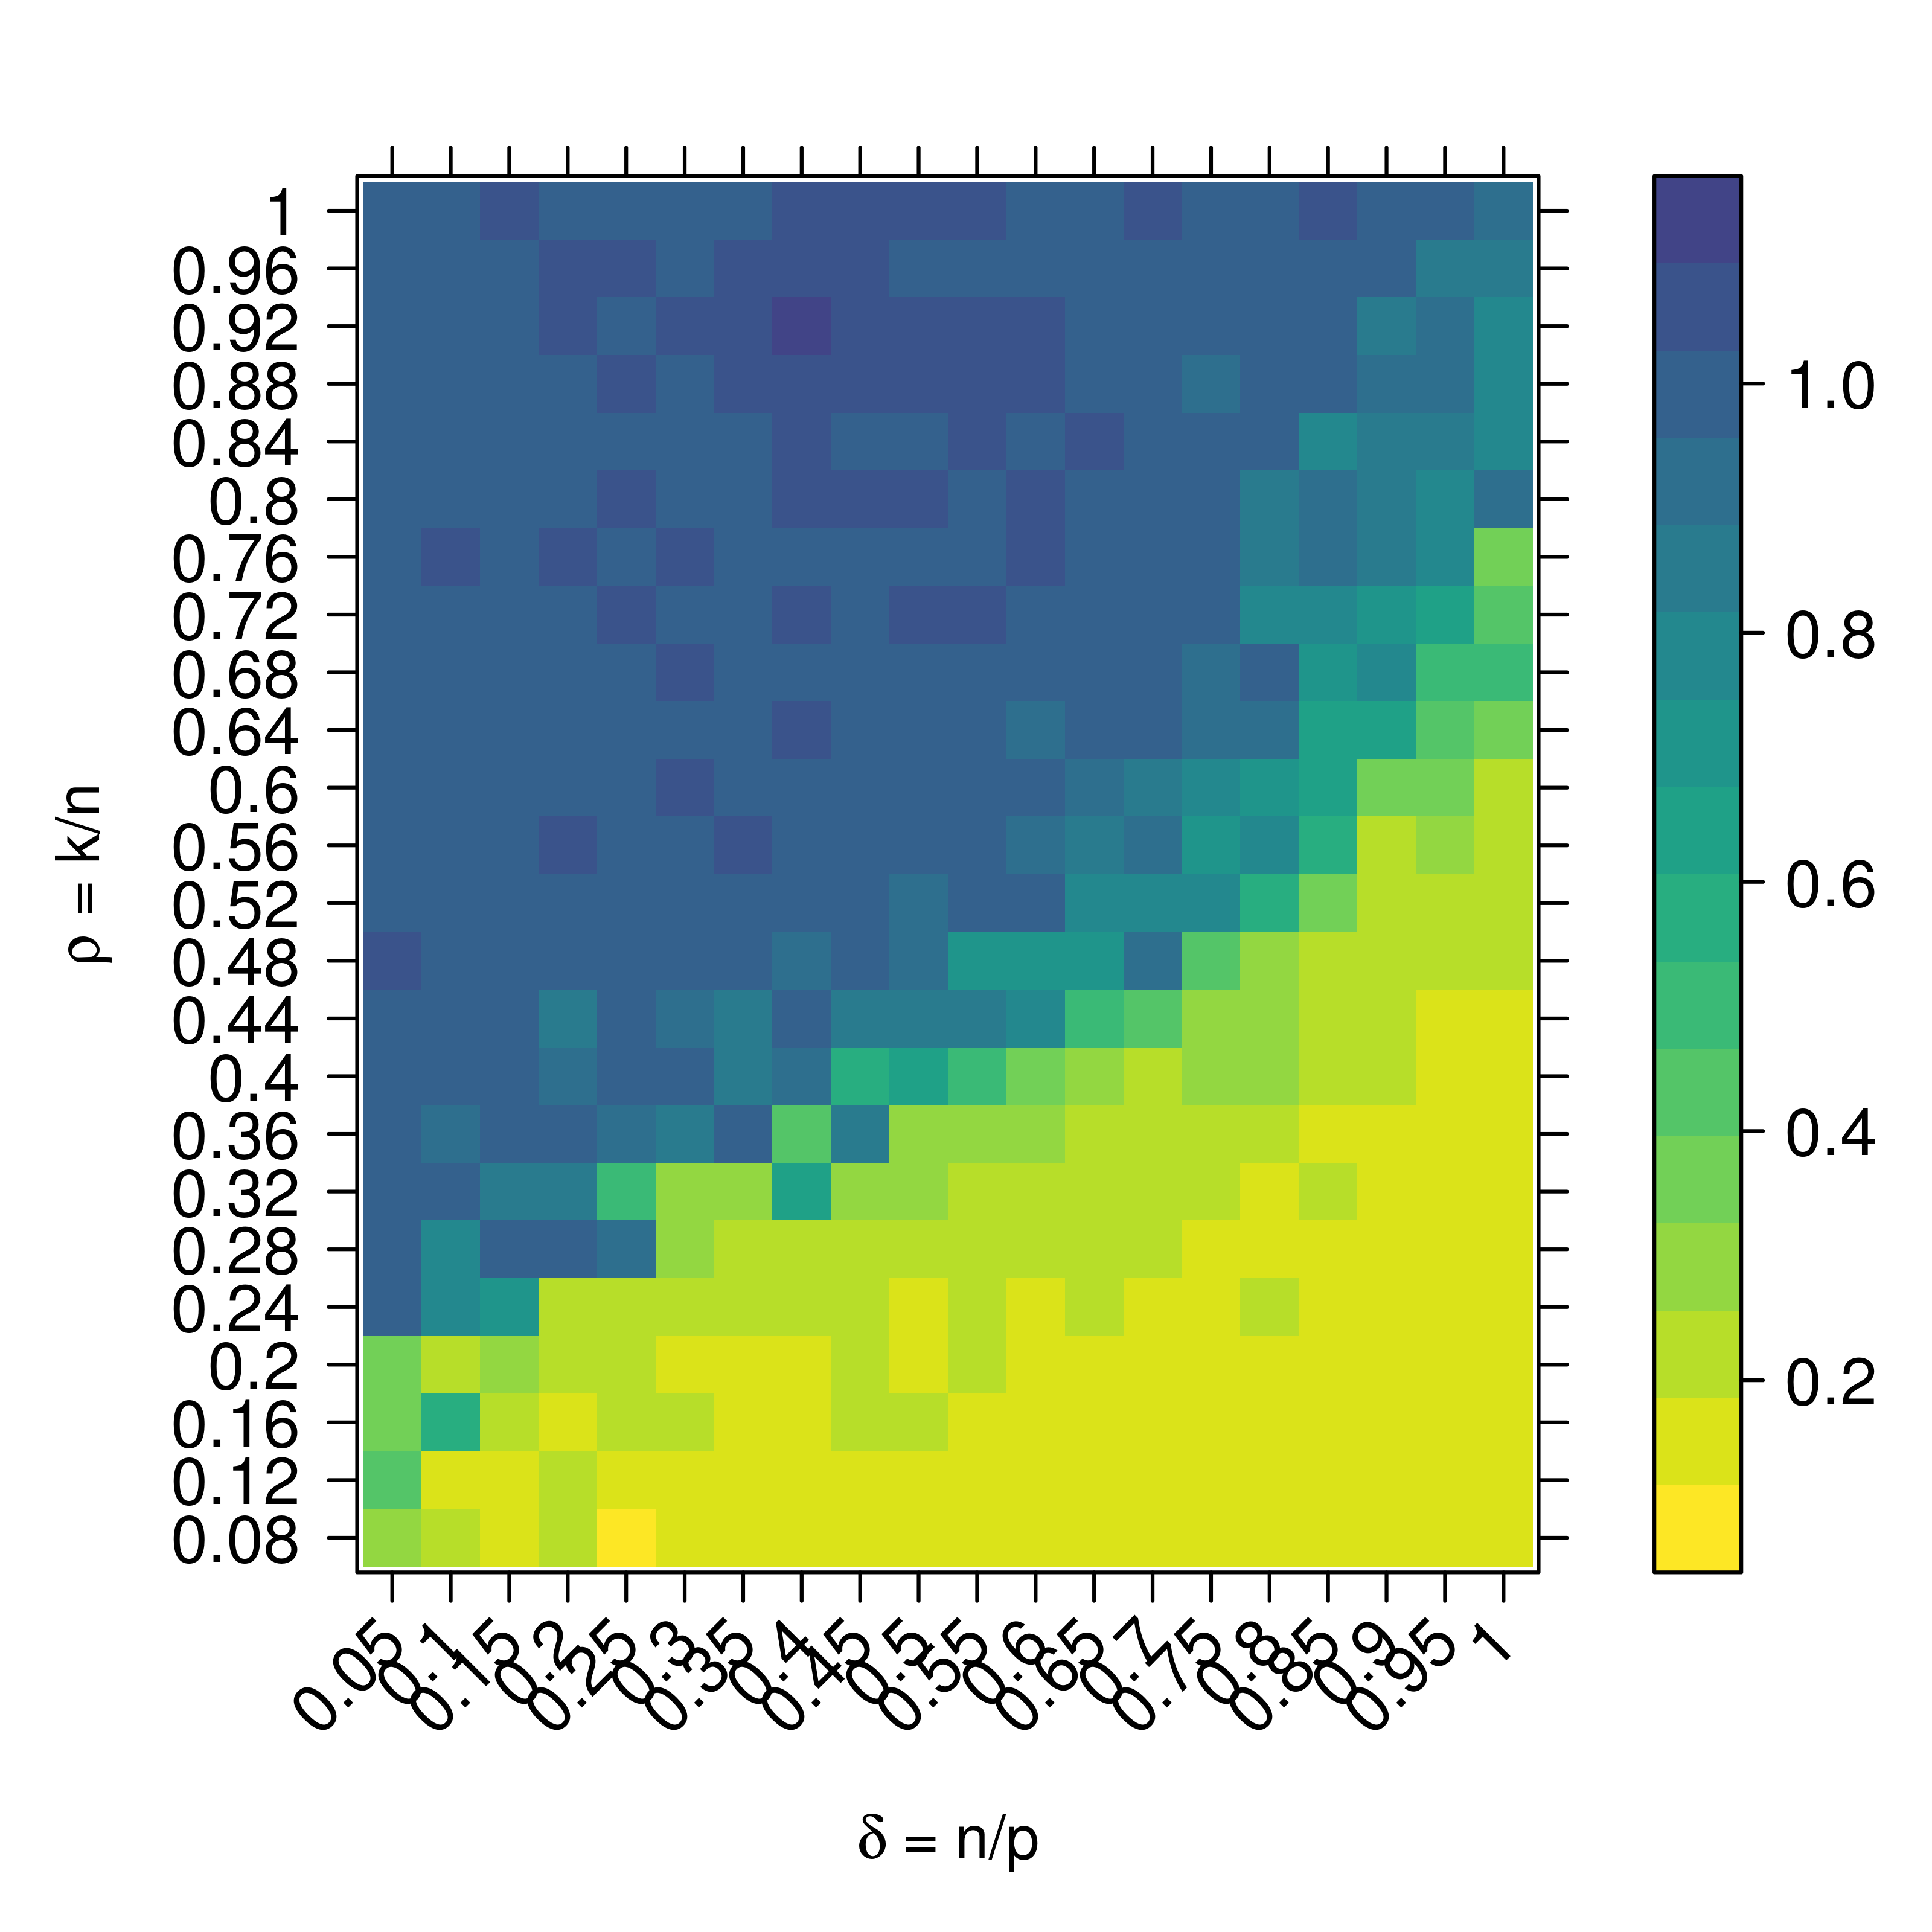
\includegraphics[totalheight=6cm]{./figs/error_Stodden_FDR.png}
       \caption{The error measure.}
       \label{figure:error_Stodden_FDR.png}
%       \vspace{4ex}
     \end{subfigure} 
     \begin{subfigure}[t]{0.5\linewidth}
       \centering
       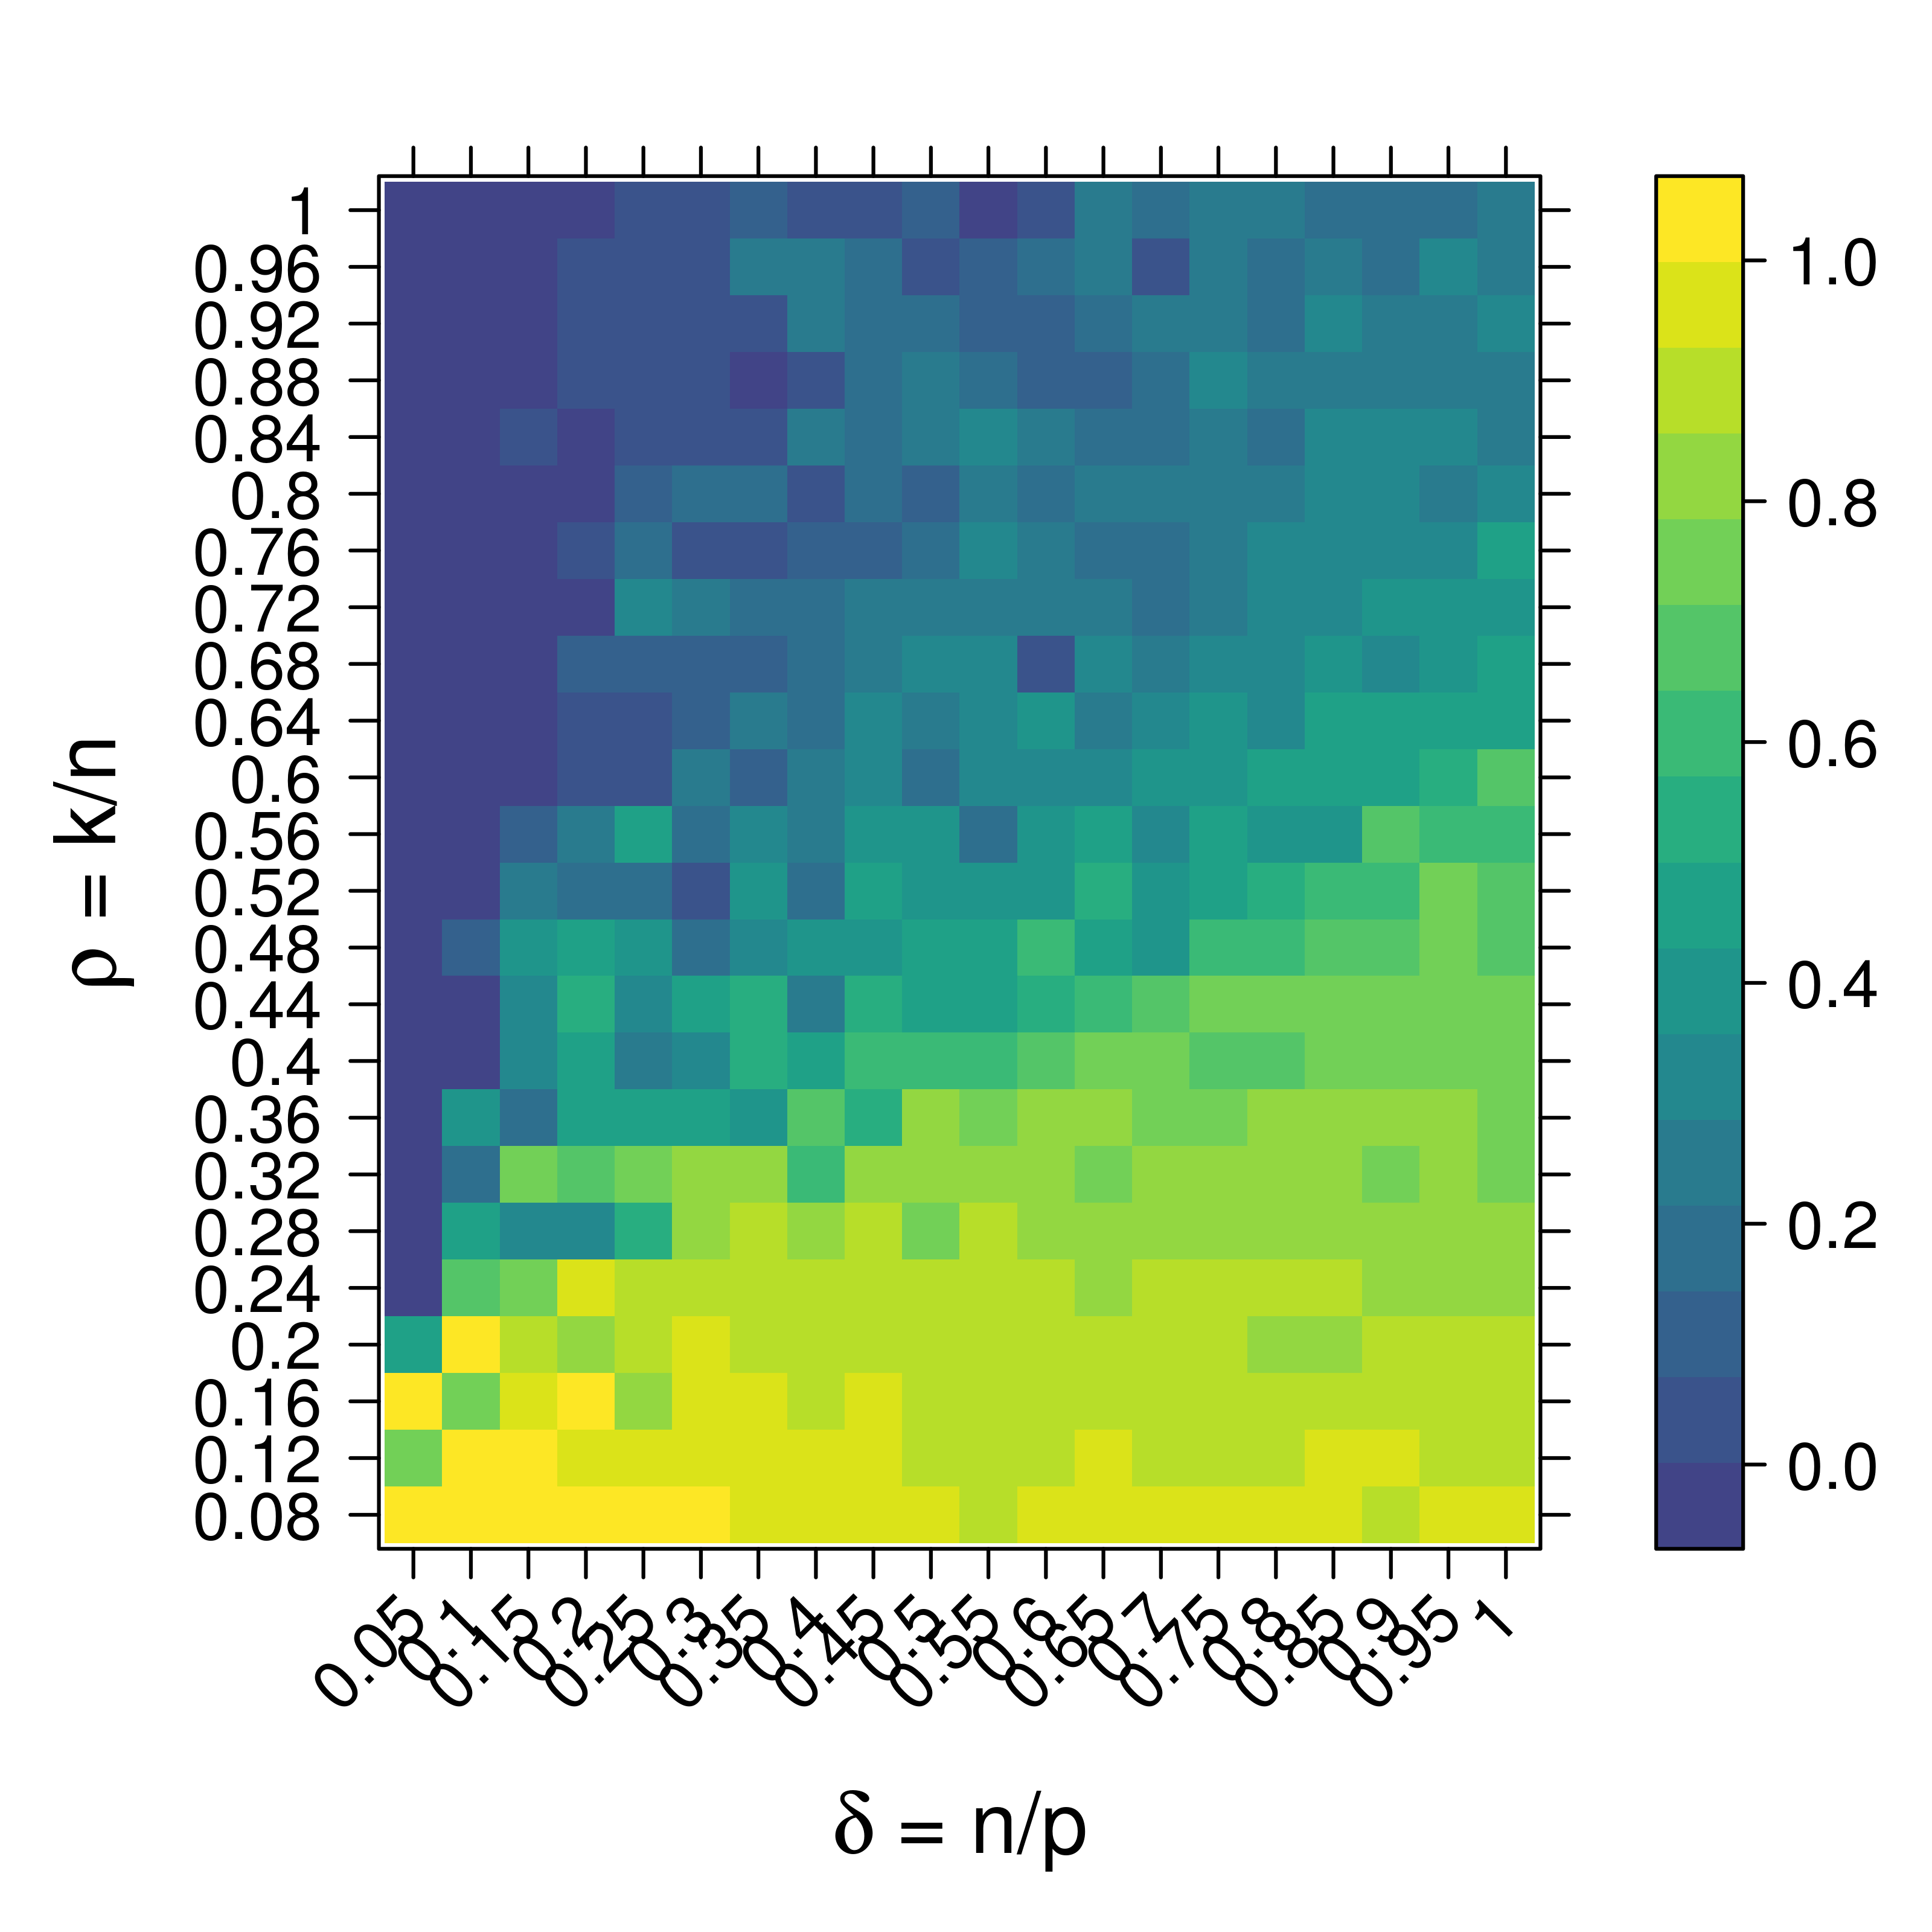
\includegraphics[totalheight=6cm]{./figs/rbo_Stodden_FDR.png}
       \caption{The RBO measure}
       \label{figure:rbo_Stodden_FDR.png}
     \end{subfigure} 
     \caption{Forward stepwise variable selction with a false discovery rate stopping criteria.}
       \label{figure:error_Stodden_FDR.png}
%   \end{adjustwidth}
 \end{figure}

 \begin{figure}[tbhp] 
     \begin{subfigure}[t]{0.5\linewidth}
       \centering
       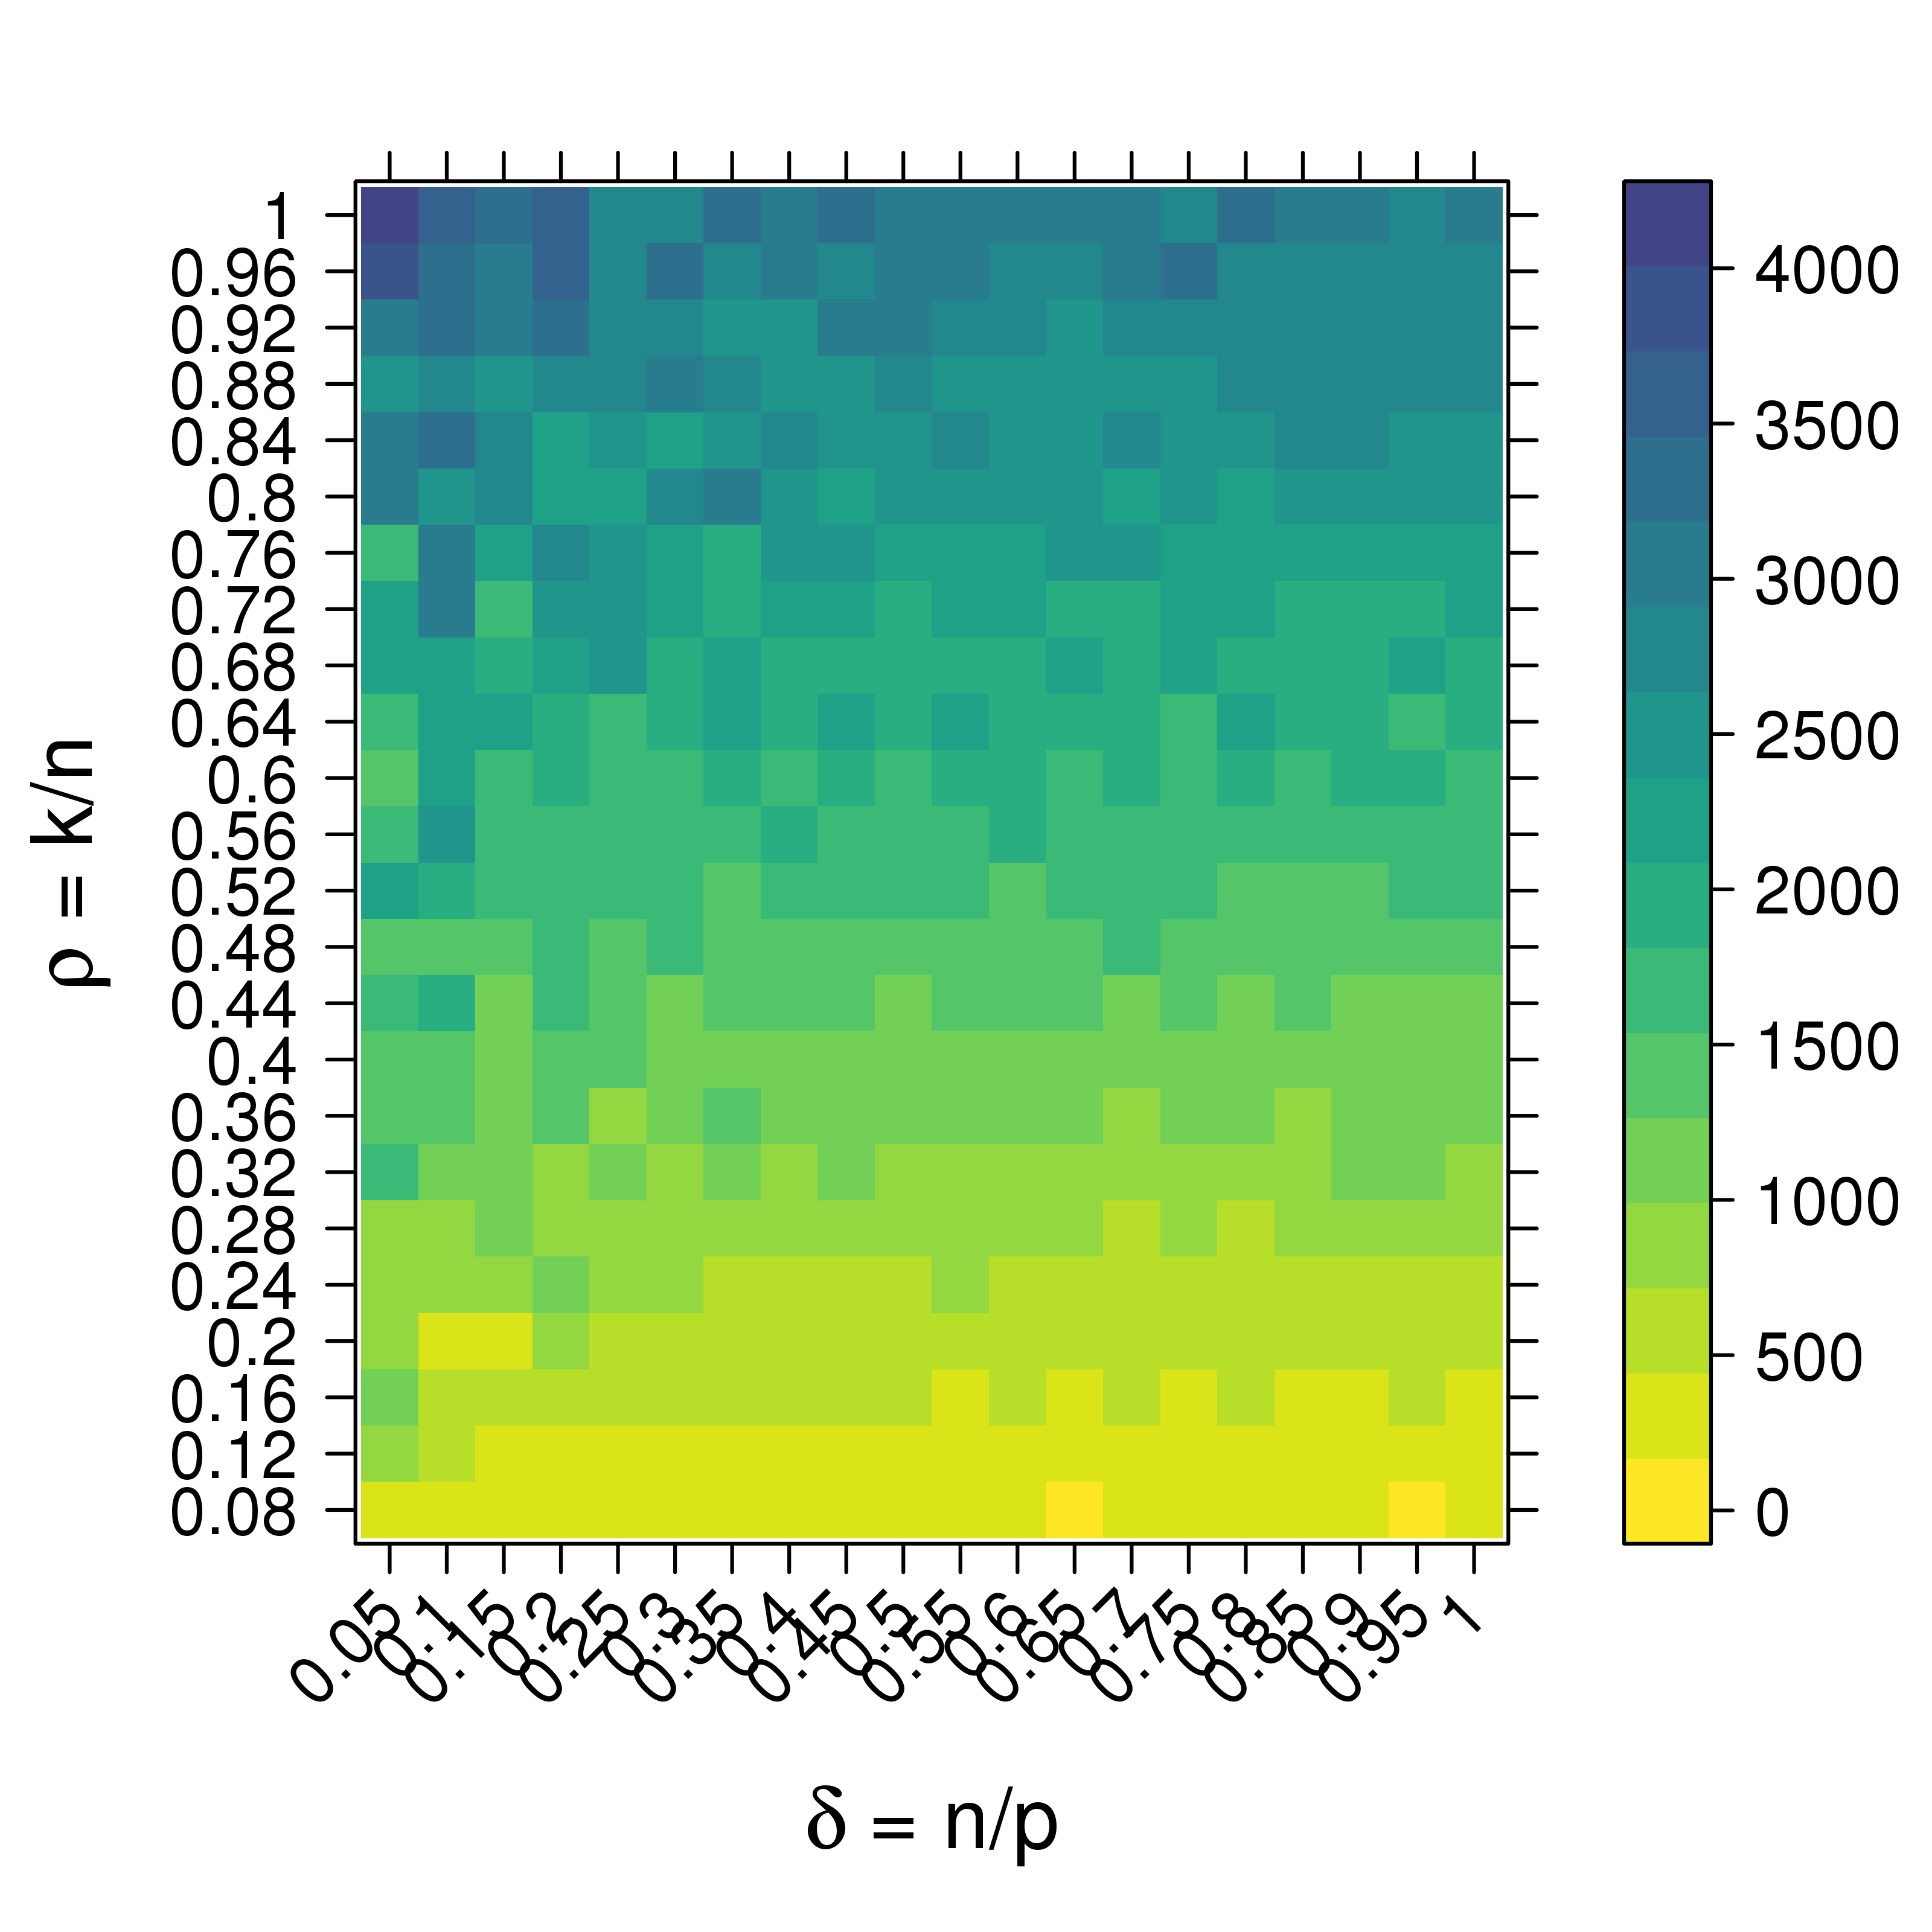
\includegraphics[totalheight=6cm]{./figs/ranger_error_Stodden_simulation.png}
       \caption{Stepwise with FDR stopping criteria. $p=200$, $n$ and $k$ variable. }
       \label{figure:ranger_error_Stodden_simulation.png}
       \vspace{4ex}
     \end{subfigure} 
     \begin{subfigure}[t]{0.5\linewidth}
       \centering
       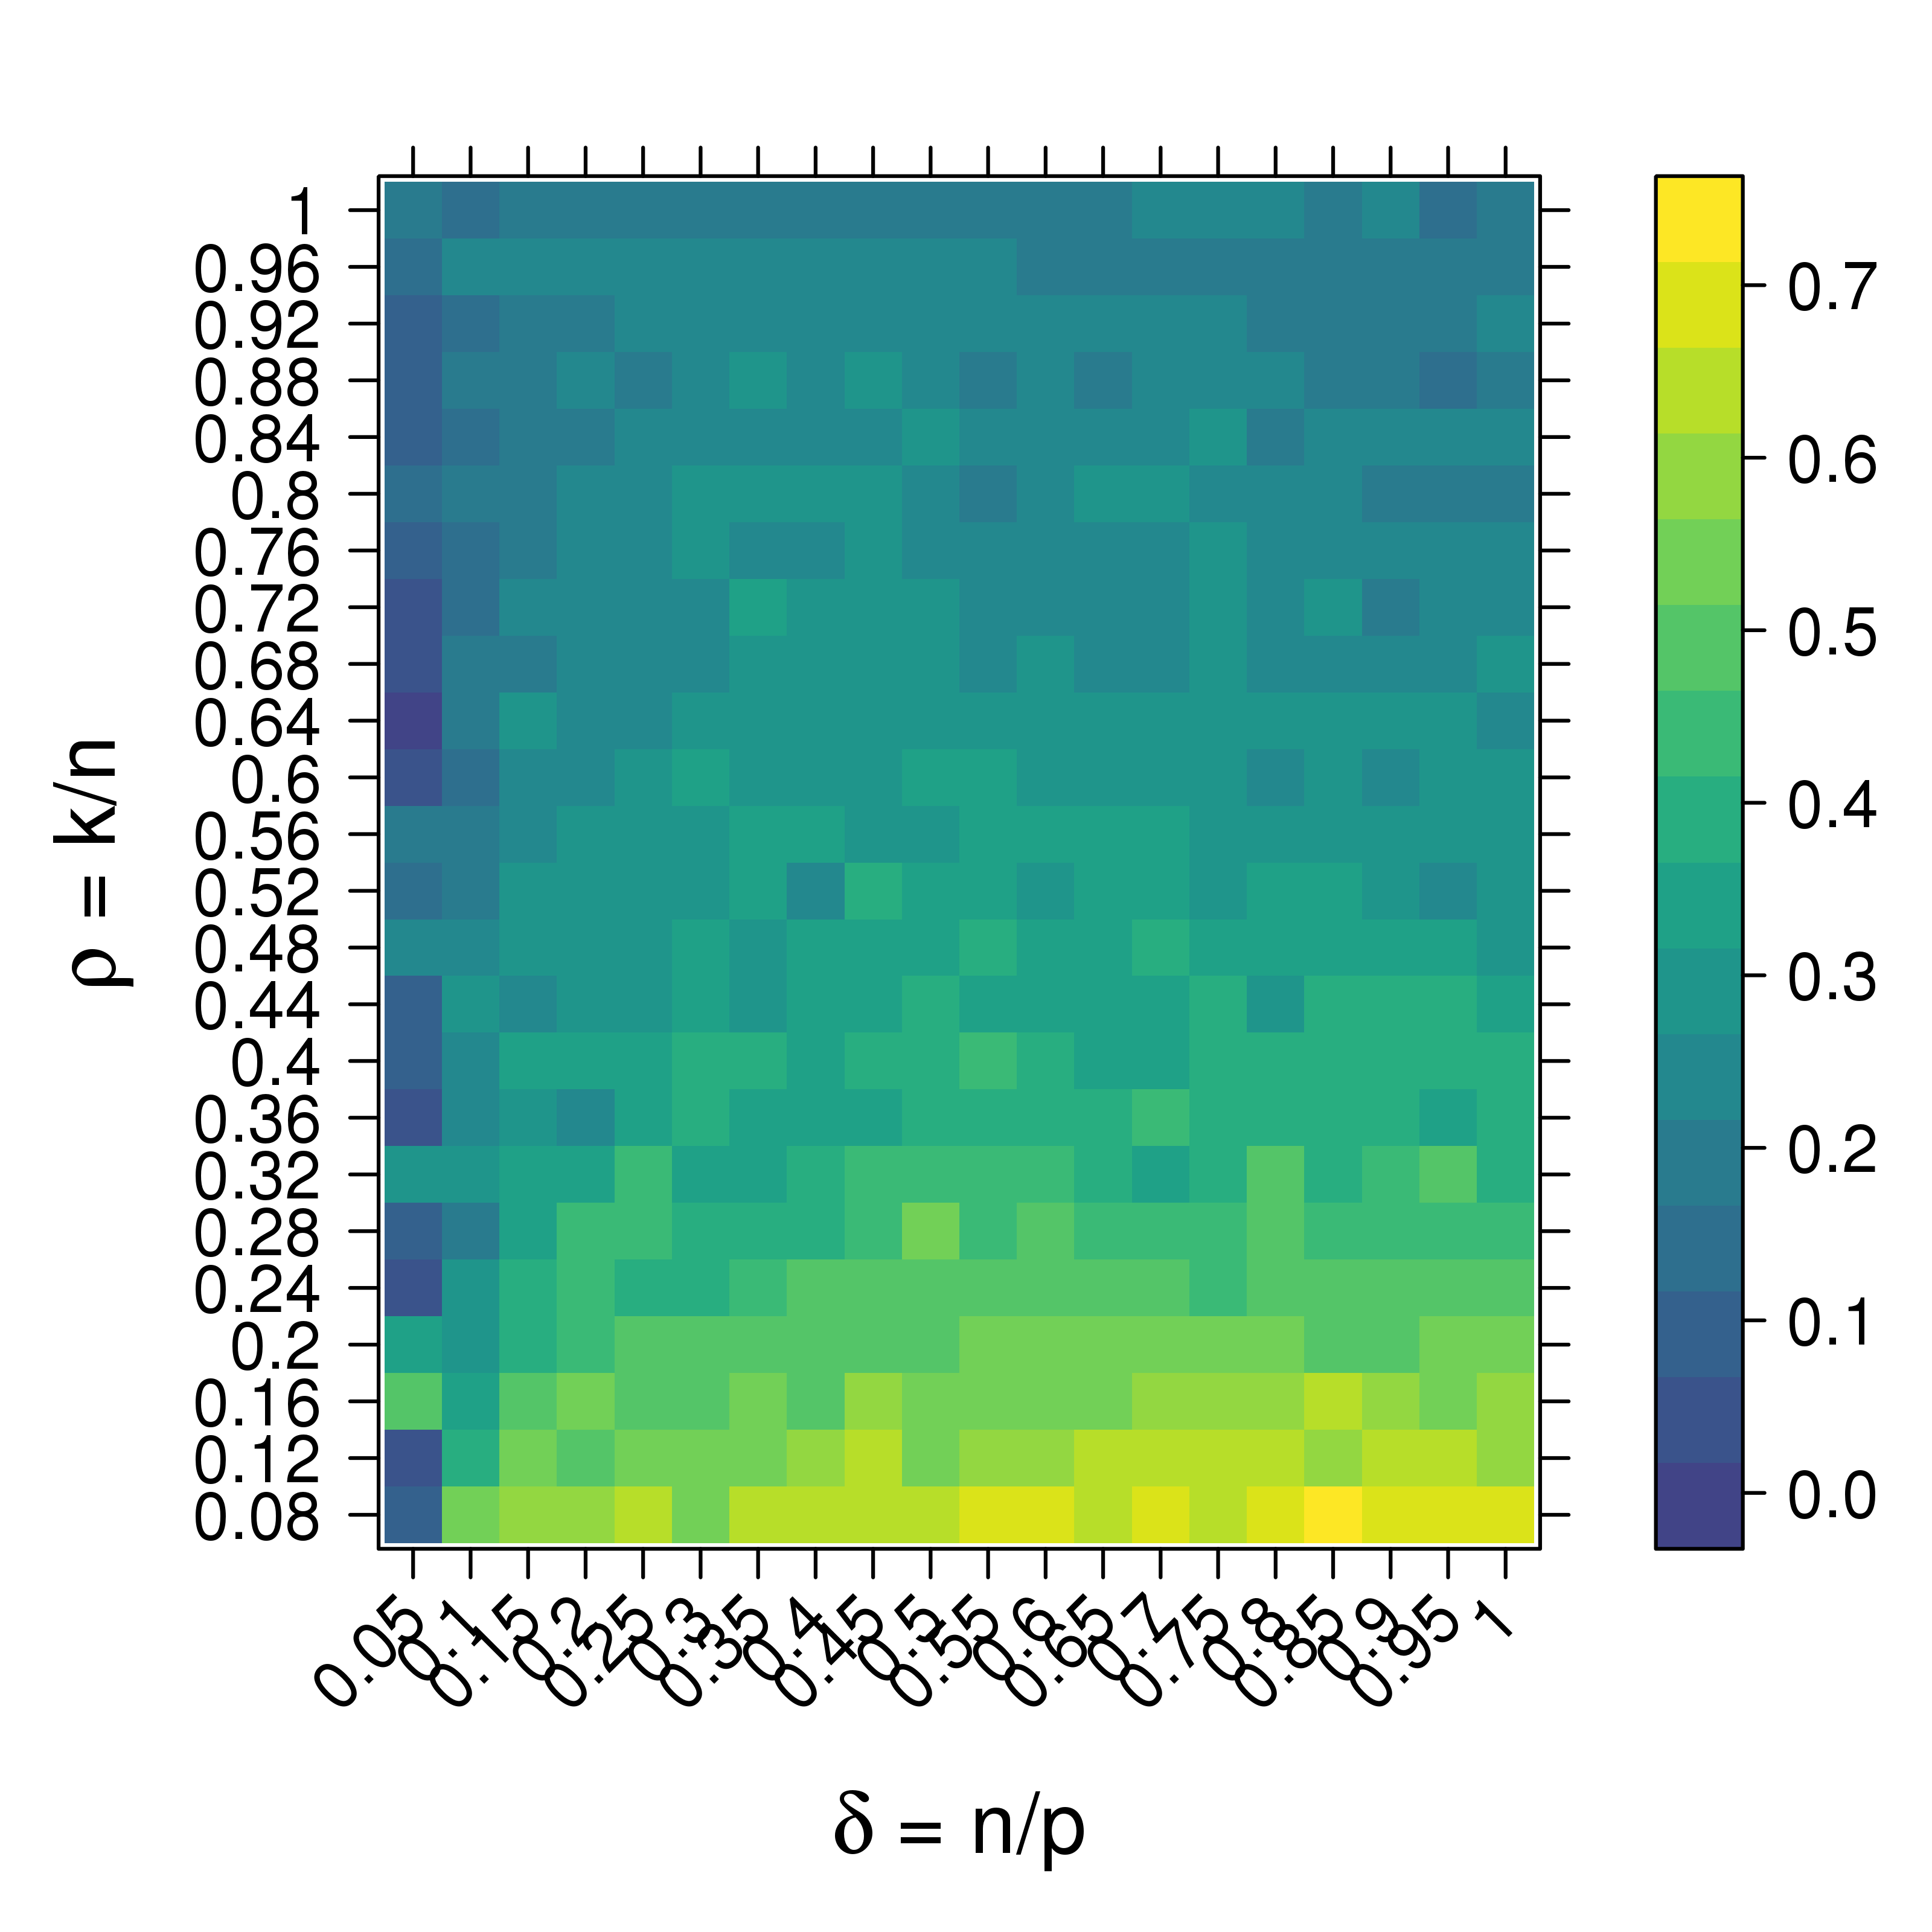
\includegraphics[totalheight=6cm]{./figs/ranger_rbo_Stodden_simulation.png}
       \caption{RBO}
       \label{figure:ranger_rbo_Stodden_simulation.png}
     \end{subfigure} 
     \caption{}
 \end{figure}


\subsection{RF on the simulation}

We have seen no work on the question of such a phase transition in the case of classification problems. Still it amy be
instructive to consider the implications of the pahse transition for our work. As \cursedforest is designed for
extremely large numbers of variables it is likely to be operating in difficult regions of the figure where the ratio
$\delta = n/p$ is small. In the simulated example in section \ref{***} the underdeterminedness $\delta = 0.002$ and the
sparsity $\rho =2\times 10^{-6}$

We have used a random forest on the same simulation as figure \ref{**}.  The Donoho-Tanner phase transition arises in
recovering the $\beta$ in data generated by a linear model. However, in a decision tree (random forest) we are fitting a
non-linear model and there is no notion of estimating the $\beta$. Becsaue of this we have evaluted the performance of
the random forest using the RBO measure on the variable importance.

We note that while a random forest is a long way from an all-seubsets search, it is a limited combinatorial search of
the feature space. As such it may perform outside of the bounds of the phase transition. 
  combinatorial search.

Fig~\ref{} shosw the OOB prediction error and the RBO error for a random forest with 10000 trees and the \mtry value set
to the default for a regression problem (depending on $n$). It shows no evidence of following the shape of the
Donoho-Tanner phase transition.


\subsection{Conclusion}

As \cursedforest is designed for extremely large numbers of variables it is likely to be operating in difficult regions of the figure.
We note that the examples we are considering lie on the extreme left of the plot, close to the origin. So there are
limits to what can be recovered in the presence of noise. However in the case of data that is both big and wide,
\cursedforest and other VariantSpark methods may provide a useful tool.

The existence of the  Donoho-Tanner phase transition is a salutary warning. There are likely to be limits, both
computational and logical, to the recovery of signals from noisy data. \cursedforest  is a contribution to addressing the
practical limits but the logical limits will still apply. However in the case of data that is both big and wide,
\cursedforest and other VariantSpark methods may provide a useful tool.



\bibliography{./CursedForest.bib}

\end{document}



